We extensively compare the \sys\/ prototype to RocksDB -- a mature industry-leading KV-store implementation  -- under a variety of scenarios. \remove{RocksDB is used as storage layer of multiple popular SQL and NoSQL databases, e.g., MyRocks~\cite{MyRocks} (incarnation of MySQL) and MongoRocks~\cite{MongoRocks} (incarnation of MongoDB). RocksDB is an LSM-tree that is highly optimized for both read and write scenarios. For example, its compaction scheduling policies are highly tuned to minimize impact on mainstream data access.} We use the most recent RocksDB release 5.17.2, available Oct 24, 2018.  
It is worth noting that RocksDB's performance improved significantly during the last two years, primarily through 
optimized LSM compaction algorithms~\cite{CallaghanCompaction}.   

\subsection{Setup}

\paragraph{Testbed.} We employ a C++ implementation~\cite{Cpp-YCSB} of a widely popular 
YCSB~\cite{YCSB} benchmarking platform. 
YCSB provides a framework for KV-store comparisons, through a set of common data access API's and standard workloads. 
Most modern KV-stores implement  YCSB adapter API's. The platform decouples data access from workload generation, 
thereby providing common ground for backend comparison. 

A workload is defined by a combination of get, put, and scan accesses, as well as by a synthetic distribution of keys and values. 
YCSB provides a set of benchmark workloads inspired by real-life applications, and allows developing new ones through workload 
generation API's. A typical YCSB instance stress-tests the backend KV-store through a pool of concurrent worker threads that drive identical
workloads. %It aggregates the key performance metrics for the scenario under test.  

Our hardware is a 12-core Intel Xeon 5 machine with 4TB SSD disk. Unless otherwise stated, the driver application 
exercises 12 workers in all experiments. In order to guarantee a fair memory allocation to all KV-stores, we run each 
experiment within a Linux container with 16 GB RAM. 

\paragraph{Metrics.} At the high level, we study the throughput and tail latency metrics produced by YCSB. 
In order to explain the results, we also explore the system write amplification (bytes written to storage over 
bytes passed from application) and read amplification (bytes read from storage over bytes passed to application), 
as well as the number of read and write system calls. The OS performance counters are retrieved from the Linux
proc filesystem. 

\paragraph{Data.} We scale the dataset size from 4 GB to 64 GB, in order to exercise multiple locality 
scenarios with respect to the available RAM. Similarly to the published RocksDB benchmarks, we use 
10-byte keys that YCSB pads with a fixed 4-byte prefix (effectively, 14-byte keys), and 800-byte values. 
The data is stored uncompressed. 

\paragraph{Workloads.} We leverage multiple workloads: 

\begin{enumerate}
\item {\em Zipf}. The key frequencies are sampled from the heavy-tailed Zipf distribution, 
following the description in~\cite{Gray:1994:QGB:191839.191886}, with $\theta = 0.8$. 
The key locations are sampled uniformly at random from the whole data range. Zipf exhibits 
medium temporal locality (e.g., the most popular key's frequency is approximately $0.7\%$), 
and no spatial locality. This is a standard YCSB workload that captures a multitude of use cases 
-- e.g., a web page cache distribution by URL. 

\item {\em Zipf-range}. Similar to Zipf ($\theta=0.8$), except that we sample the key's $14$ most significant bits
(MSBs) rather than the complete key. The remainder of the key sampled uniformly at random. Zipf-range exhibits
a workload of high spatial locality, e.g., message threads~\cite{Borthakur:2011:AHG:1989323.1989438}. 

\item {\em Latest}. New KV-pairs are inserted in sequential key order; the most recently inserted ones are 
the  most popular (the sampled key's position wrt the most recent key is distributed Zipf). This is a 
standard YCSB workload of medium spatial and temporal locality that exhibits, e.g., status updates and reads. 

\end{enumerate}

The workloads exercise different mixes of puts, gets, and scans. We use standard YCSB scenarios 
(A to E) that capture write-savvy ($50\%$ puts) to read-savvy ($95\%-100\%$ gets or scans) settings. 
In order to stress the system even more on the write side, we introduce a new workload, named 
YCSB-P, comprised of $100\%$ puts. It captures a heavy-duty data load scenario (e.g., from an 
external data pipeline). 

\paragraph{Evaluation methodology.} Each experiment consists of two stages. The first stage builds 
the dataset, by filling an initially empty store with an sequence of KV-pairs, ordered by key. The second 
phase exercises the specific scenario; all worker threads follow the same access pattern. Most experiments 
perform 80 million data accesses. The experiments that run scans perform 4 to 16 million accesses, depending 
on the scan size. We run 5 experiments for each data point, and present the median metric measurement. 

\paragraph{Configuration.} 
We only present the performance metrics in asynchronous logging mode -- as synchronous logging 
is approximately 10 times slower, thereby trivializing the results of every scenario that includes puts. 

We allocate a quota of 13.5 GB RAM (out of the 16 GB container) to the munk and row caches, 
and split it between the two at a $2:1$ ratio. 

The Bloom filters for munk-less funks are partitioned 16-way.  
We set the \sys\/ chunk size limit to 10 MB, and the rebalance threshold factor to $0.7$ -- i.e., 
most chunks are bound by 7 MB (i.e., approximately 7000 KV-pairs per chunk). The funk log
size limit is 2 MB for write intensive workloads, and 512 KB for other workloads.

We tune all RocksDB runtime parameters in accordance with its system performance guide~\cite{RocksDBPerf}.   

\subsection{Results}

\begin{figure*}[tb]
\centering
\begin{subfigure}{0.3\linewidth}
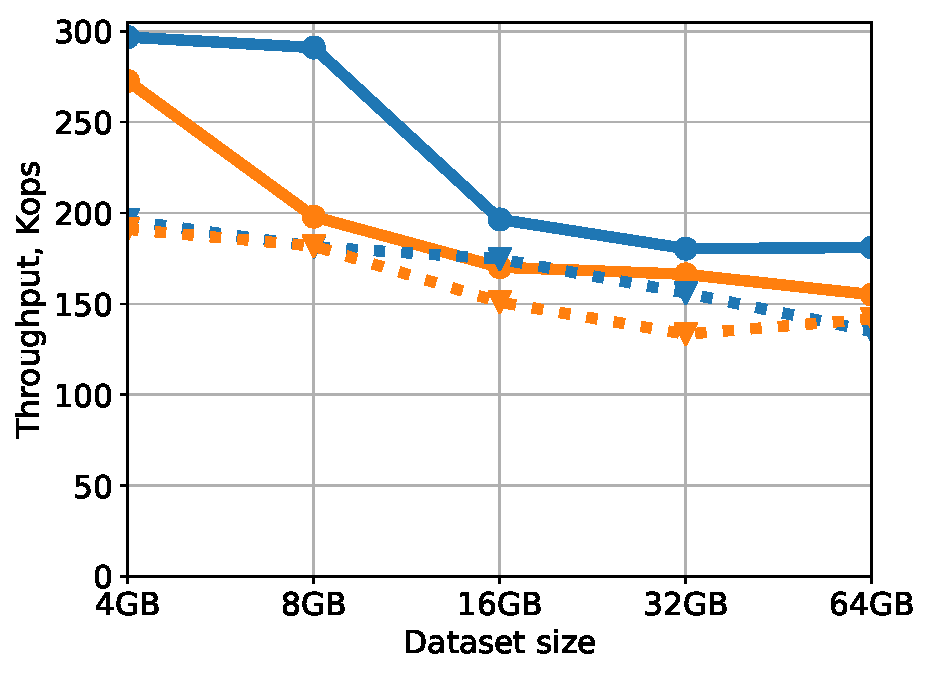
\includegraphics[width=\textwidth]{figs/Workload_P_line.pdf}
\caption{YCSB-P}
\label{fig:throughput:p}
\end{subfigure}
\begin{subfigure}{0.3\linewidth}
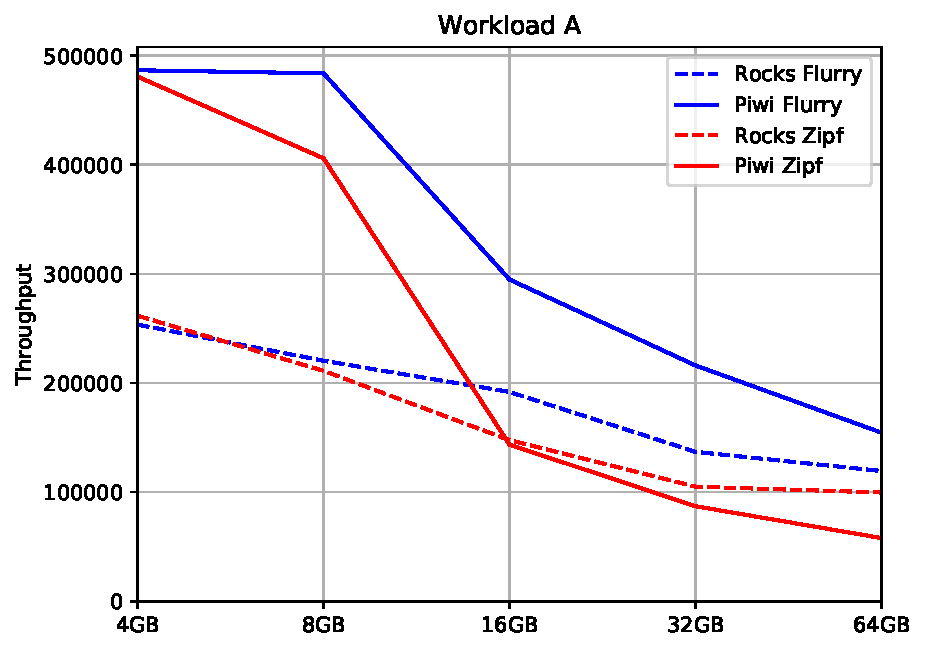
\includegraphics[width=\textwidth]{figs/Workload_A_line.pdf}
\caption{YCSB-A}
\label{fig:throughput:a}
\end{subfigure}
\begin{subfigure}{0.3\linewidth}
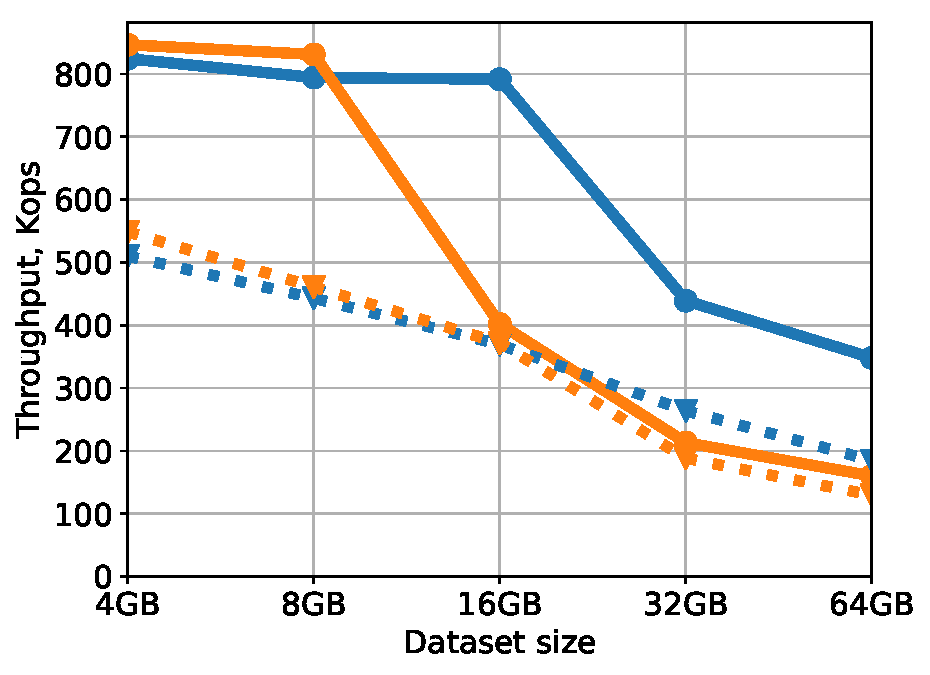
\includegraphics[width=\textwidth]{figs/Workload_C_line.pdf}
\caption{YCSB-C}
\label{fig:throughput:c}
\end{subfigure}
%\begin{subfigure}{0.3\linewidth}
%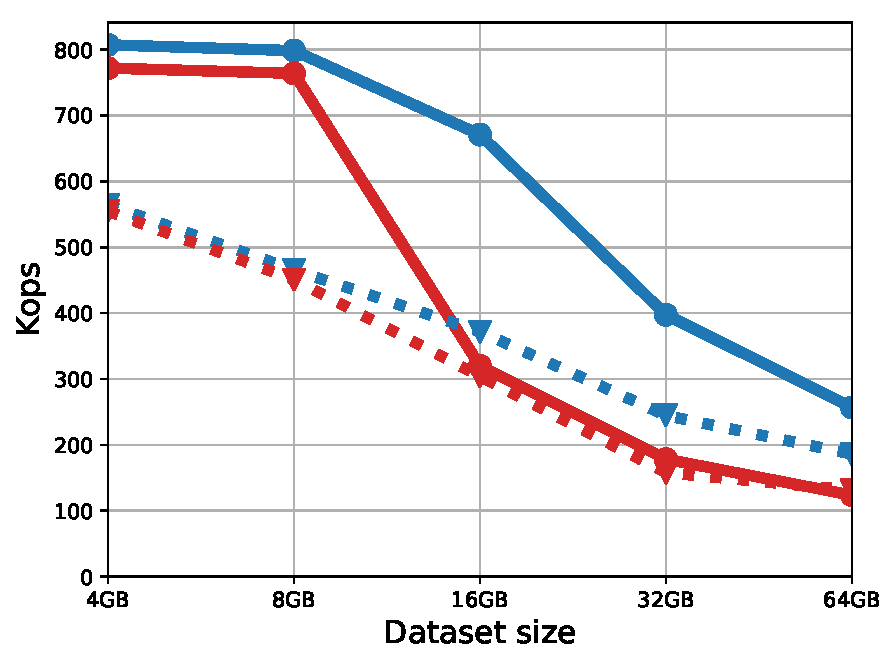
\includegraphics[width=\textwidth]{figs/Workload_B_line.pdf}
%\caption{YCSB-B}
%\label{fig:throughput:b}
%\end{subfigure}
%\begin{subfigure}{0.3\linewidth}
%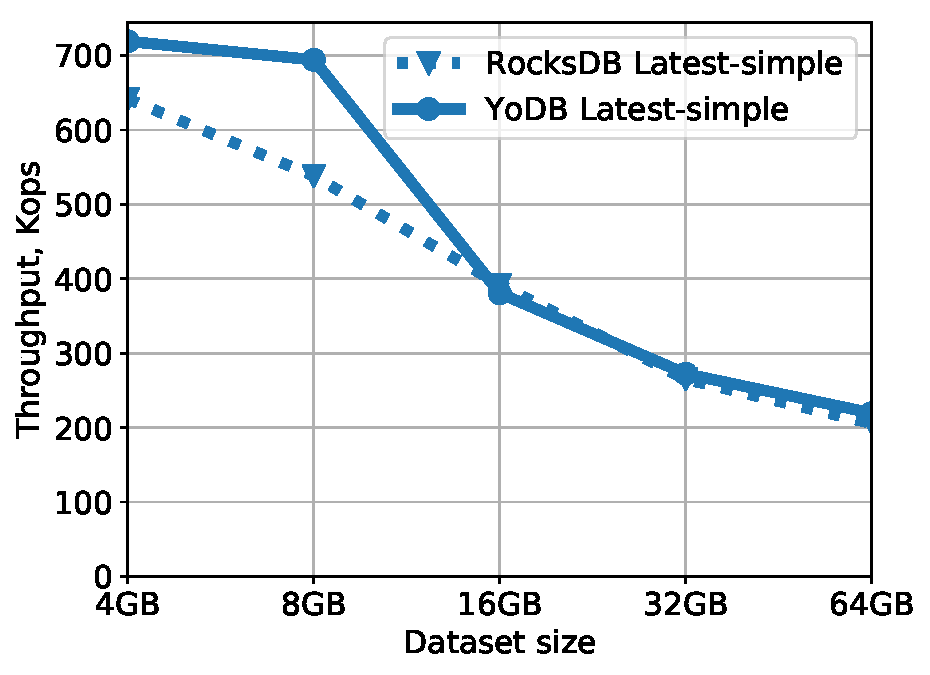
\includegraphics[width=\textwidth]{figs/Workload_D_line.pdf}
%\caption{YCSB-D}
%\label{fig:throughput:d}
%å\end{subfigure}
\begin{subfigure}{0.3\linewidth}
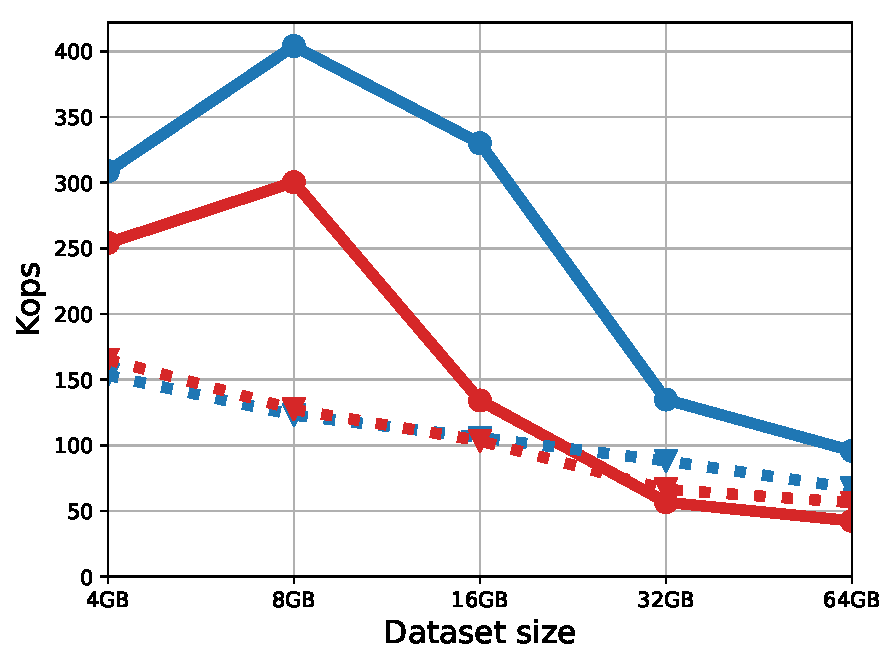
\includegraphics[width=\textwidth]{figs/Workload_E-_line.pdf}
\caption{YCSB-E10}
\label{fig:throughput:e10}
\end{subfigure}
\begin{subfigure}{0.3\linewidth}
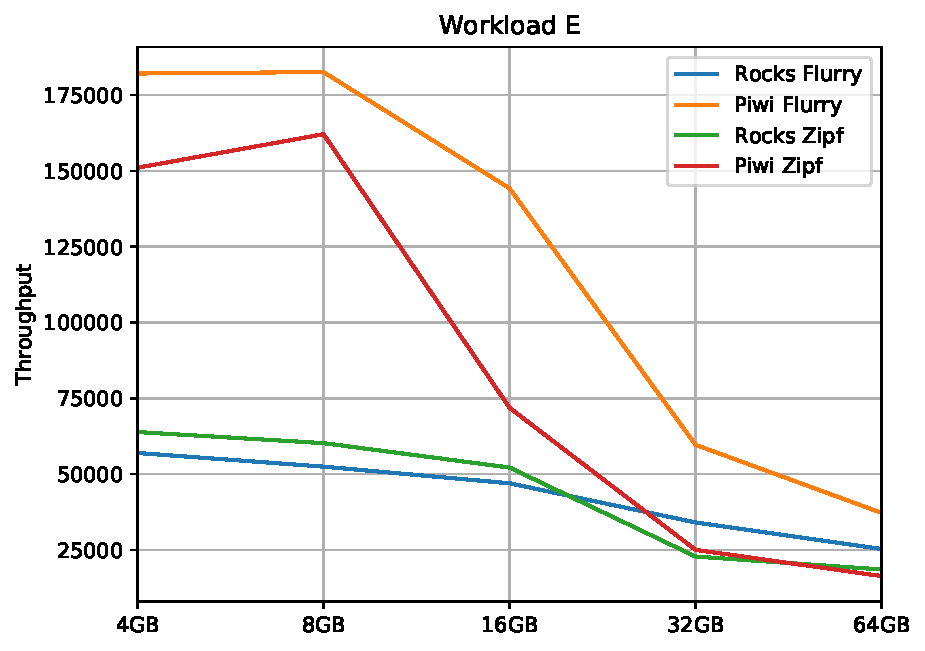
\includegraphics[width=\textwidth]{figs/Workload_E_line.pdf}
\caption{YCSB-E100}
\label{fig:throughput:e100}
\end{subfigure}
\begin{subfigure}{0.3\linewidth}
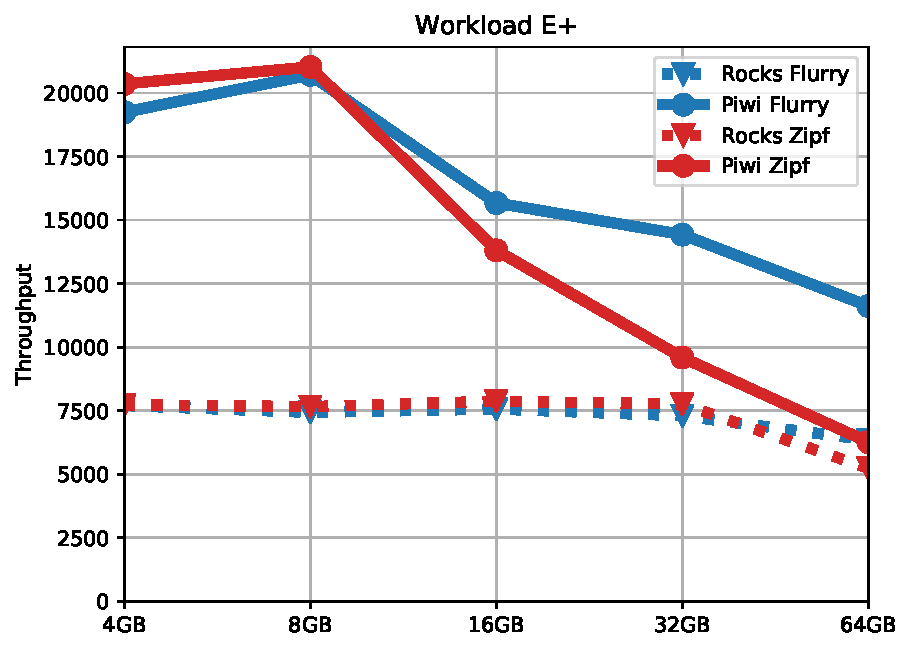
\includegraphics[width=\textwidth]{figs/Workload_E+_line.pdf}
\caption{YCSB-E1000}
\label{fig:throughput:e1000}
\end{subfigure}
\caption{\bf{\sys\/ versus RocksDB throughput, under multiple workloads and scaling dataset sizes.}}
\label{fig:throughput}
\end{figure*}

\paragraph{YCSB-P (100\% put, Zipf and Zipf-range distributions).} 
\sys's throughput is $30\%$ to $60\%$ above RocksDB's under Zipf-range, 
and $10\%$ to $50\%$ under Zipf (Figure~\ref{fig:throughput:p}). 
\sys\ achieves better throughput for Zipf-range compared to Zipf, 
thanks to high spatial locality. In contrast, RocksDB's write performance 
is relatively insensitive to the distribution, which is typical for LSM data stores.

This workload's bottleneck is the persistent data reorganization 
(funk rebalances for \sys, compactions for RocksDB). The overhead
manifests in disk write rates, which \sys\/ reduces through better use of spatial locality. 
For small datasets (8 GB or less), \sys\/ accommodates all puts in munks, which alleviates 
funk rebalances altogether. For big datasets, only part of the chunks are cached, hence 
funk rebalances start occurring. However, they mostly happen to munk-less 
(torso) chunks. Hence, they incur less I/O than RocksDB's compactions, which do not 
distinguish between hot and cold data. 

Table~\ref{fig:writeamp} corroborates the above observations, by comparing 
\sys's write amplification to RocksDB's. \sys\/ reduces the disk write rate dramatically, 
with the largest gain observed for big datasets (e.g., $1.29$ versus $2.92$ for the 64 GB 
database under Zipf-range). As a nice by-product, \sys\/ is also more 
efficient with respect to disk wear.  

\paragraph{YCSB-A (50\% put, 50\% get), Zipf and Zipf-range distributions).}
YCSB-A  is particularly challenging for \sys\/ because it exercises a high contention between gets and puts. 
\sys\/ achieves $1.3$x to $2.2$x throughput versus RocksDB under Zipf-range (Figure~\ref{fig:throughput:a}), 
thanks to better exploitation of spatial locality. Under the Zipf workload, it is faster than RocksDB for small
datasets that fit in memory, and slower for big datasets.  

The bottleneck in this scenario is the on-disk search part of gets, primarily the linear search in funk logs 
that keep filling up due to concurrent puts. In-memory searches are three orders of magnitude 
faster. Figure~\ref{fig:readstat:dist} depicts the distribution of gets by the storage hierarchy component 
that fulfilled the request, whereas Figure~\ref{fig:readstat:lat} presents the disk search latencies by component. 
For example, for the 64 GB dataset, $1.9\%$ of gets are served from logs under Zipf-range, versus $4.0\%$ under Zipf. 
The log search latencies are $1.7$ ms vs $4.4$ ms. This happens because under Zipf the puts are more dispersed, 
hence the funks are (1) cached less effectively by the OS, and (2) rebalanced less frequently, i.e., the logs grow longer
and searching them becomes slower. 

% Bloom filter efficiency ... 

Naturally, the efficiency of in-memory caching is paramount. In the same example, the RAM hit rate is 
$90.5\%$ versus $79\%$ for Zipf. The row cache becomes instrumental as spatial locality drops --
e.g., it serves $32.8\%$ of gets for Zipf versus $12.4\%$ for Zipf-range. 

\paragraph{YCSB-E (5\% put, 95\% scan, Zipf and Zipf-range distributions).}
This workload is the best for \sys, since it is most sensitive to spatial locality
that the system has been designed for. 
We experiment with short-to-medium scans, with the number of KV-pairs to iterate through 
sampled uniformly between 1 and 10, 100, and 1000 rows, respectively (Figures~\ref{fig:throughput:e10}-~\ref{fig:throughput:e1000}). 
\sys\/ achieves $1.5$x to $3$x throughput versus RocksDB under Zipf-range, and even $1.5$x to 2x under Zipf, in most cases. 

Note that the scan speed is slightly higher for the 8GB dataset versus the 4GB dataset. 
Both are served in memory, however, the 4GB store has less munks, and hence, there is more contention 
betweens scans and puts, that slows down the overall progress. This phenomenon becomes insignificant 
with longer scans. 

\paragraph{YCSB-C (100\% get, Zipf and Zipf-range distributions).}  
\sys\/ achieves $1.6$x to $2.1$x throughput versus RocksDB under Zipf-range,
and up to $1.6$x under Zipf for small datasets (Figure~\ref{fig:throughput:c}).   

Since this experiment only exercises the read path, we can compare \sys's RAM caching 
efficiency to RocksDB's. Both system exploit both application-level and OS (filesystem) caches. 
Table~\ref{fig:readamp} compares the two systems' read amplification (as proxy for cache hit ratio), 
with respect to the number of read system calls and the actual disk reads.  In terms of disk I/O, RocksDB 
is slightly better -- e.g., $0.95$ versus $1.07$ for the 64 GB dataset under Zipf-range. However, it 
relies extensively on the filesystem cache, at the expense of the user-level block cache. In the same
setting, it performs almost 12 times more system calls than \sys, hence wasting the CPU resources on  
kernel-to-user data copy. RocksDB developers explain that the block cache scaling potential is limited in their
database, due to tension between its read-path and write-path RAM resources~\cite{RocksDB-default-blockcache-issue}. 
\sys, in contrast, exploits its munk cache for both reads and writes, which leads to better RAM utilization. 

\paragraph{YCSB-B and YCSB-D (5\% put, 95\% get, Zipf, Zipf-prefix and Latest distributions).} Similar to YCSB-C, 
illustration omitted due to lack of space. 

\begin{table}[th]
{\small{
\begin{tabular}{|l|c|c|c|c|c|}
\hline 
& 4GB & 8GB & 16GB & 32GB & 64GB \\
\hline 
RocksDB, Zipf-range & 1.93	& 2.15 & 2.29 & 2.54	& {\bf {2.92}}\\
\sys, Zipf-range &  1.42	 & 1.38	& 1.27	& 1.30	& {\bf {1.29}}\\
\hline 
RocksDB, Zipf & 1.94 & 2.20	& 2.69 & 3.03 &	2.77 \\ 
\sys, Zipf & 1.41& 1.37	& 1.15	& 1.13	& 1.31 \\
\hline 
\end{tabular}
}}
%\centering
%\hspace{0.05\linewidth}
%\begin{subfigure}{0.3\linewidth}
%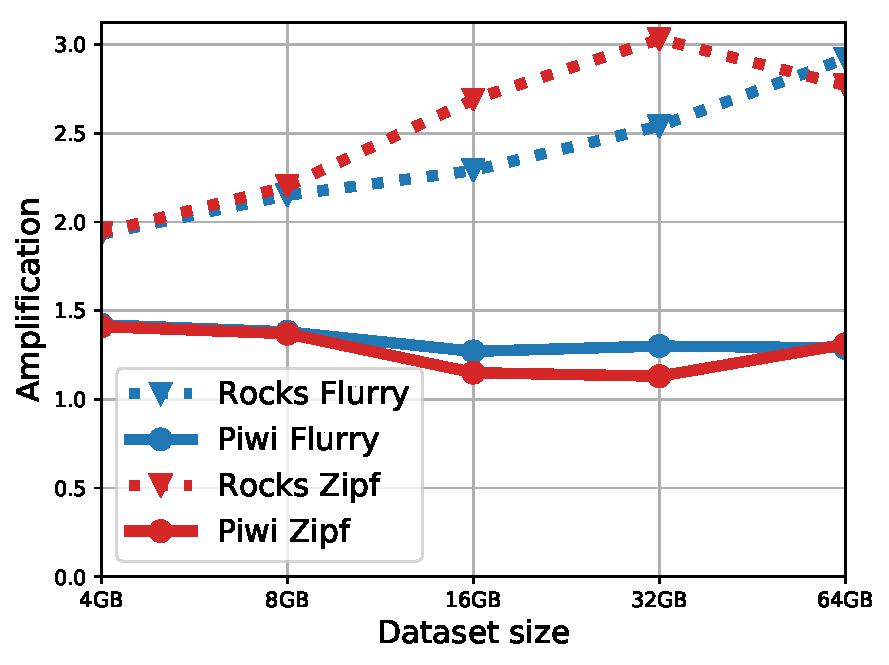
\includegraphics[width=0.3\textwidth]{figs/P_write_amplification_disk_line.pdf}
%\caption{YCSB-P}
%\label{fig:writeamp:p}
%\end{subfigure}
%\hspace{0.05\linewidth}
%\begin{subfigure}{0.3\linewidth}
%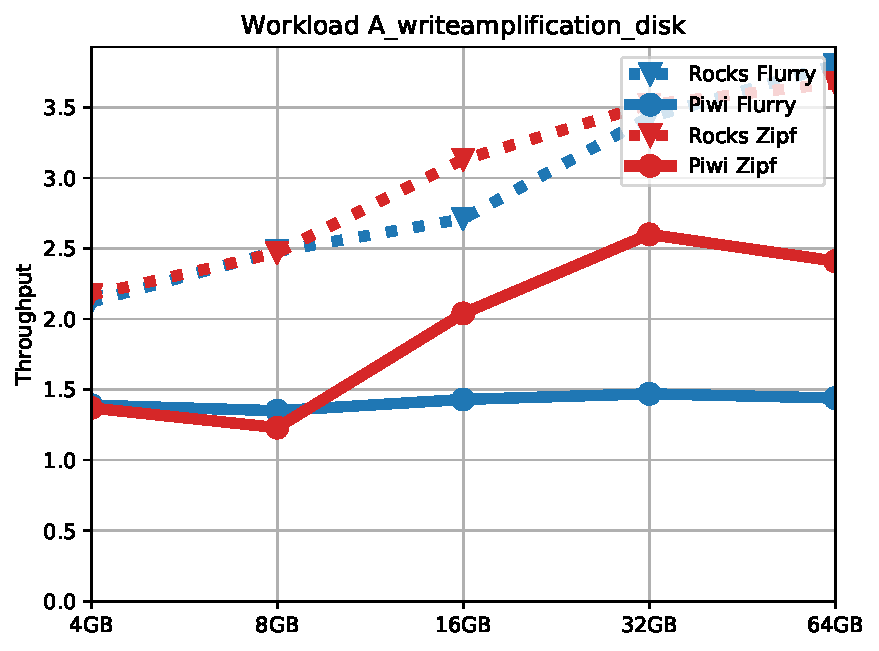
\includegraphics[width=\textwidth]{figs/Workload_A_writeamplification_disk_line.pdf}
%\caption{YCSB-A}
%\label{fig:writeamp:a}
%\end{subfigure}
\caption{\bf{\sys\/ versus RocksDB write amplification, under the write-only workload (YCSB-P) and scaling dataset sizes.}}
\label{fig:writeamp}
\end{table}

\begin{figure}
\centering
%\hspace{0.05\linewidth}
\begin{subfigure}{0.49\linewidth}
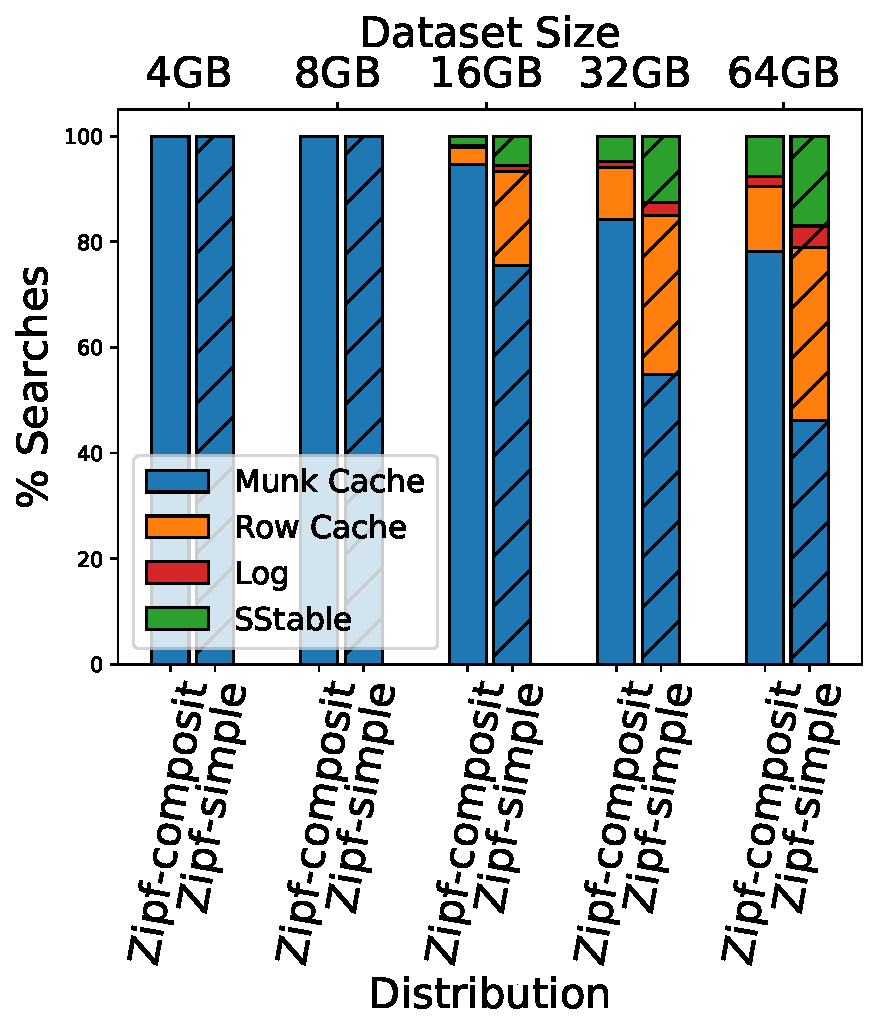
\includegraphics[width=\textwidth]{figs/Time_percentage_A.pdf}
\caption{Fraction of searches}
\label{fig:readstat:dist}
\end{subfigure}
%\hspace{0.05\linewidth}
\begin{subfigure}{0.49\linewidth}
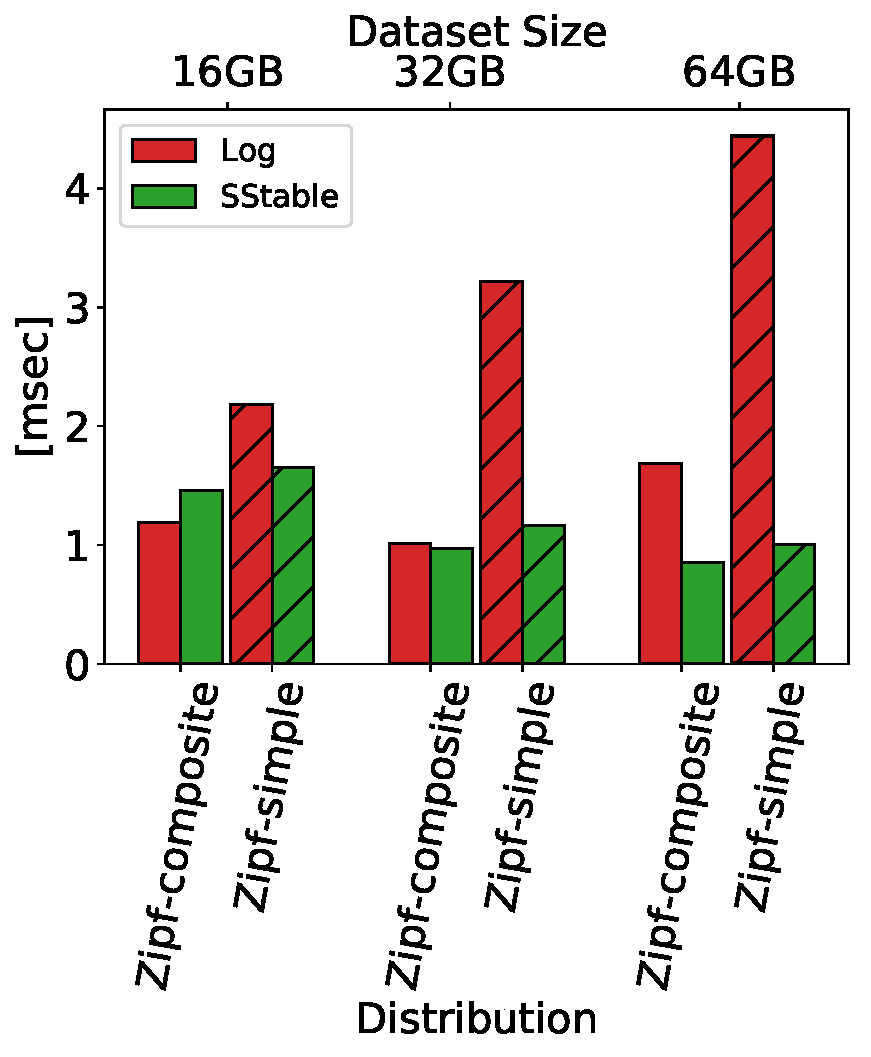
\includegraphics[width=\textwidth]{figs/Latency_A.pdf}
\caption{Disk search latency}
\label{fig:readstat:lat}
\end{subfigure}
\caption{\bf{\sys\/ {\em get\/} operation statistics by the serving component, under the mixed read-write workload (YCSB-A) and scaling dataset sizes.}}
\label{fig:readstat}
\end{figure}

%\paragraph{YCSB-D (5\% put, 95\% get, Latest distribution).} Similar to YCSB-C, illustration omitted due to lack of space. 

\section{Insights}

\paragraph{Vertical scalabiliy.} 
Figure~\ref{fig:scalability} illustrates the \sys's throughput scaling for the 64 GB dataset, under the Zipf and Zipf-range 
distributions. We exercise the YCSB-A, YCSB-C and YCSB-P scenarios, with 1 to 16 worker threads.  

\begin{figure}[th]
\centering
%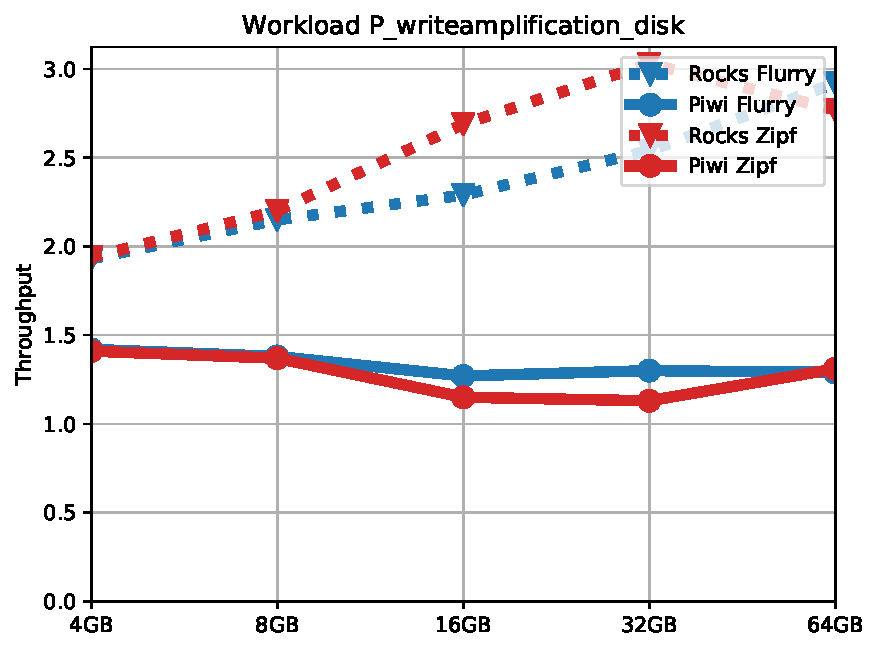
\includegraphics[width=0.3\textwidth]{figs/Workload_P_writeamplification_disk_line.pdf}
\caption{\bf{\sys\/ scalability with the number of application threads.}}
\label{fig:scalability}
\end{figure}

\begin{table}
{\small{
\begin{tabular}{|l|c|c|c|c|c|}
\hline 
& 4GB & 8GB & 16GB & 32GB & 64GB \\
\hline 
RocksDB, bytes &  0.05 &	0.11 & 0.20 & 0.47 & 0.95\\
\sys, bytes &  0.0 &	0.0 &	0.11	& 0.80	& 1.07 \\
\hline 
RocksDB, syscall & 3.84	& 4.01	& 4.14	& 4.28	& {\bf {4.37}} \\ 
\sys, syscall  & 0.0 & 0.0	& 0.10 & 0.24 & {\bf {0.41}} \\
\hline 
\end{tabular}
}}
\caption{\bf{\sys\/ versus RocksDB read amplification, in terms of bytes and system calls, 
under the read-only workload (YCSB-C), Zipf-range distribution and scaling dataset sizes.}}
\label{fig:readamp}
\end{table}

\paragraph{Funk-log configuration.} 
We explore the system throughput sensitivity to funk-log configuration parameters, for the 64 GB dataset, 
under the YCSB-A scenario. 

Table~\ref{fig:wal:sz} depicts the throughput dependency on the log size limit. Here, too low a threshold (e.g., 128 KB) 
causes frequent funk rebalances, which degrades the performance more than 3-fold. On the other hand, too high a threshold (4 MB) 
lets the logs grow bigger, and slows down all types of reads. Our experiments are therefore tuned to 2 MB logs under write-intensive 
workloads. In other scenarios, funk rebalances are infrequent, hence we set a relatively aggressive 512 KB threshold to avoid high tail
latencies. 

\begin{table*}
\centering
\begin{subfigure}{0.55\linewidth}
{\small{
\begin{tabular}{|l|c|c|c|c|c|c|}
\hline 
& 128KB & 256KB & 512KB & 1MB & 2MB & 4MB\\
\hline 
Zipf-range & 50.2	& 55.5 & 80.7	& 134.1 & {\bf {157.5}} & 149.5 \\
Zipf & 27.8	& 30.9 & 36.1	& 58.3	& {\bf {68.3}}	& 68.1 \\
%\hline 
%YCSB-E, Zipf-range & 29.1	& 36.4 & 36.9	& 37.3	& {\inred{30.4}} & 	37.1 \\
%YCSB-E, Zipf & 16.1 & 16.3 &	15.8	& 15.8 &	16.4 &	15.8 \\
\hline
\end{tabular}
}}
\caption{Throughput (Kops) vs log size}
\label{fig:wal:sz}
\end{subfigure}
%\hspace{0.09\linewidth}
\begin{subfigure}{0.35\linewidth}
{\small{
\begin{tabular}{|l|c|c|c|c|c|}
\hline 
& 1 & 2 & 4 & 8 & 16\\
\hline 
Zipf-range & 134.7 & 133.5 & 140.1 & 152.5 & {\bf {157.4}} \\
Zipf & 36.3 & 39.2 & 46.3 & 56.0 & {\bf {59.9}} \\
\hline 
\end{tabular}
}}
\caption{Throughput (Kops) vs Bloom filter split factor}
\label{fig:wal:bf}
\end{subfigure}
\caption{\bf{\sys\/ throughput, under the mixed read-write workload (YCSB-A), 64GB dataset, and varying funk log configuration parameters.}}
\label{fig:wal}
\end{table*}

Table~\ref{fig:wal:bf} depicts the throughput dependency on the Bloom filter split factor. 
Partitioning to 16 mini-filters gives the best result, which explains the default parameter choice. 
